% Created by tikzDevice version 0.6.2-92-0ad2792 on 2013-11-12 07:32:40
% !TEX encoding = UTF-8 Unicode
\documentclass[12pt, mainfont = Minion,     mainscale = 1.0, sansfont = Myriad,     sansscale = MatchLowercase, monofont = Consolas,   monoscale = MatchLowercase, mathfont = MinionMath, mathscale = 1.0]{mtikzfig}
\begin{document}

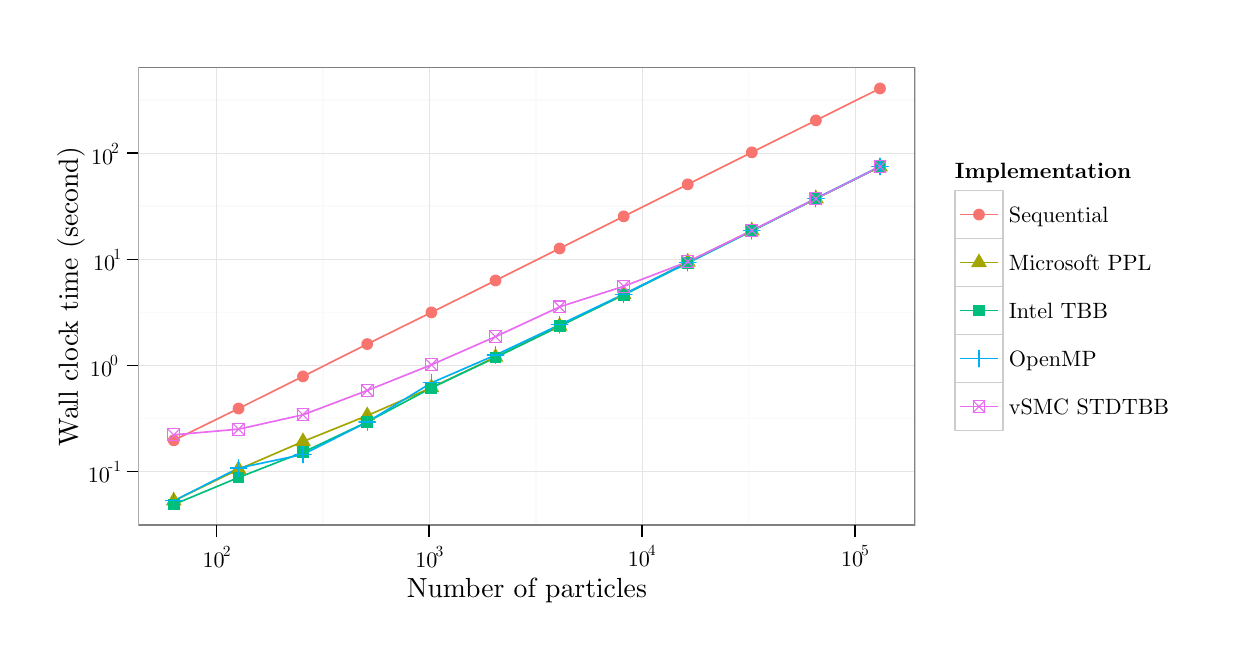
\begin{tikzpicture}[x=1pt,y=1pt]
\definecolor[named]{fillColor}{rgb}{1.00,1.00,1.00}
\path[use as bounding box,fill=fillColor,fill opacity=0.00] (0,0) rectangle (433.62,216.81);
\begin{scope}
\path[clip] (  0.00,  0.00) rectangle (433.62,216.81);
\definecolor[named]{drawColor}{rgb}{1.00,1.00,1.00}
\definecolor[named]{fillColor}{rgb}{1.00,1.00,1.00}

\path[draw=drawColor,line width= 0.6pt,line join=round,line cap=round,fill=fillColor] (  0.00,  0.00) rectangle (433.62,216.81);
\end{scope}
\begin{scope}
\path[clip] ( 40.02, 37.00) rectangle (320.74,202.36);
\definecolor[named]{fillColor}{rgb}{1.00,1.00,1.00}

\path[fill=fillColor] ( 40.02, 37.00) rectangle (320.74,202.36);
\definecolor[named]{drawColor}{rgb}{0.98,0.98,0.98}

\path[draw=drawColor,line width= 0.6pt,line join=round] ( 40.02, 37.22) --
	(320.74, 37.22);

\path[draw=drawColor,line width= 0.6pt,line join=round] ( 40.02, 75.57) --
	(320.74, 75.57);

\path[draw=drawColor,line width= 0.6pt,line join=round] ( 40.02,113.92) --
	(320.74,113.92);

\path[draw=drawColor,line width= 0.6pt,line join=round] ( 40.02,152.27) --
	(320.74,152.27);

\path[draw=drawColor,line width= 0.6pt,line join=round] ( 40.02,190.62) --
	(320.74,190.62);

\path[draw=drawColor,line width= 0.6pt,line join=round] (106.67, 37.00) --
	(106.67,202.36);

\path[draw=drawColor,line width= 0.6pt,line join=round] (183.58, 37.00) --
	(183.58,202.36);

\path[draw=drawColor,line width= 0.6pt,line join=round] (260.49, 37.00) --
	(260.49,202.36);
\definecolor[named]{drawColor}{rgb}{0.90,0.90,0.90}

\path[draw=drawColor,line width= 0.2pt,line join=round] ( 40.02, 56.39) --
	(320.74, 56.39);

\path[draw=drawColor,line width= 0.2pt,line join=round] ( 40.02, 94.74) --
	(320.74, 94.74);

\path[draw=drawColor,line width= 0.2pt,line join=round] ( 40.02,133.09) --
	(320.74,133.09);

\path[draw=drawColor,line width= 0.2pt,line join=round] ( 40.02,171.44) --
	(320.74,171.44);

\path[draw=drawColor,line width= 0.2pt,line join=round] ( 68.22, 37.00) --
	( 68.22,202.36);

\path[draw=drawColor,line width= 0.2pt,line join=round] (145.13, 37.00) --
	(145.13,202.36);

\path[draw=drawColor,line width= 0.2pt,line join=round] (222.03, 37.00) --
	(222.03,202.36);

\path[draw=drawColor,line width= 0.2pt,line join=round] (298.94, 37.00) --
	(298.94,202.36);
\definecolor[named]{drawColor}{rgb}{0.97,0.46,0.43}

\path[draw=drawColor,line width= 0.6pt,line join=round] ( 52.78, 67.69) --
	( 76.20, 79.19) --
	( 99.48, 90.80) --
	(122.70,102.48) --
	(145.89,113.92) --
	(169.05,125.44) --
	(192.21,137.02) --
	(215.37,148.62) --
	(238.52,160.19) --
	(261.68,171.76) --
	(284.83,183.31) --
	(307.98,194.84);
\definecolor[named]{drawColor}{rgb}{0.64,0.65,0.00}

\path[draw=drawColor,line width= 0.6pt,line join=round] ( 52.78, 45.82) --
	( 76.20, 57.21) --
	( 99.48, 67.26) --
	(122.70, 76.63) --
	(145.89, 86.75) --
	(169.05, 97.78) --
	(192.21,109.02) --
	(215.37,120.35) --
	(238.52,132.14) --
	(261.68,143.41) --
	(284.83,155.00) --
	(307.98,166.55);
\definecolor[named]{drawColor}{rgb}{0.00,0.75,0.49}

\path[draw=drawColor,line width= 0.6pt,line join=round] ( 52.78, 44.51) --
	( 76.20, 54.26) --
	( 99.48, 63.37) --
	(122.70, 74.35) --
	(145.89, 86.65) --
	(169.05, 97.61) --
	(192.21,108.93) --
	(215.37,120.24) --
	(238.52,131.79) --
	(261.68,143.35) --
	(284.83,155.00) --
	(307.98,166.61);
\definecolor[named]{drawColor}{rgb}{0.00,0.69,0.96}

\path[draw=drawColor,line width= 0.6pt,line join=round] ( 52.78, 45.82) --
	( 76.20, 57.68) --
	( 99.48, 62.58) --
	(122.70, 74.30) --
	(145.89, 88.47) --
	(169.05, 98.51) --
	(192.21,109.44) --
	(215.37,120.51) --
	(238.52,131.91) --
	(261.68,143.43) --
	(284.83,155.10) --
	(307.98,166.63);
\definecolor[named]{drawColor}{rgb}{0.91,0.42,0.95}

\path[draw=drawColor,line width= 0.6pt,line join=round] ( 52.78, 69.68) --
	( 76.20, 71.72) --
	( 99.48, 76.92) --
	(122.70, 85.70) --
	(145.89, 94.98) --
	(169.05,105.15) --
	(192.21,115.92) --
	(215.37,123.34) --
	(238.52,132.23) --
	(261.68,143.50) --
	(284.83,155.00) --
	(307.98,166.57);
\definecolor[named]{fillColor}{rgb}{0.97,0.46,0.43}

\path[fill=fillColor] ( 52.78, 67.69) circle (  2.13);
\definecolor[named]{fillColor}{rgb}{0.64,0.65,0.00}

\path[fill=fillColor] ( 52.78, 49.14) --
	( 55.66, 44.16) --
	( 49.91, 44.16) --
	cycle;
\definecolor[named]{fillColor}{rgb}{0.00,0.75,0.49}

\path[fill=fillColor] ( 50.65, 42.38) --
	( 54.92, 42.38) --
	( 54.92, 46.65) --
	( 50.65, 46.65) --
	cycle;
\definecolor[named]{drawColor}{rgb}{0.00,0.69,0.96}

\path[draw=drawColor,line width= 0.4pt,line join=round,line cap=round] ( 49.77, 45.82) -- ( 55.80, 45.82);

\path[draw=drawColor,line width= 0.4pt,line join=round,line cap=round] ( 52.78, 42.80) -- ( 52.78, 48.84);
\definecolor[named]{drawColor}{rgb}{0.91,0.42,0.95}

\path[draw=drawColor,line width= 0.4pt,line join=round,line cap=round] ( 50.65, 67.54) rectangle ( 54.92, 71.81);

\path[draw=drawColor,line width= 0.4pt,line join=round,line cap=round] ( 50.65, 67.54) -- ( 54.92, 71.81);

\path[draw=drawColor,line width= 0.4pt,line join=round,line cap=round] ( 50.65, 71.81) -- ( 54.92, 67.54);
\definecolor[named]{fillColor}{rgb}{0.97,0.46,0.43}

\path[fill=fillColor] ( 76.20, 79.19) circle (  2.13);
\definecolor[named]{fillColor}{rgb}{0.64,0.65,0.00}

\path[fill=fillColor] ( 76.20, 60.52) --
	( 79.07, 55.55) --
	( 73.33, 55.55) --
	cycle;
\definecolor[named]{fillColor}{rgb}{0.00,0.75,0.49}

\path[fill=fillColor] ( 74.07, 52.13) --
	( 78.33, 52.13) --
	( 78.33, 56.40) --
	( 74.07, 56.40) --
	cycle;
\definecolor[named]{drawColor}{rgb}{0.00,0.69,0.96}

\path[draw=drawColor,line width= 0.4pt,line join=round,line cap=round] ( 73.18, 57.68) -- ( 79.22, 57.68);

\path[draw=drawColor,line width= 0.4pt,line join=round,line cap=round] ( 76.20, 54.66) -- ( 76.20, 60.69);
\definecolor[named]{drawColor}{rgb}{0.91,0.42,0.95}

\path[draw=drawColor,line width= 0.4pt,line join=round,line cap=round] ( 74.07, 69.59) rectangle ( 78.33, 73.85);

\path[draw=drawColor,line width= 0.4pt,line join=round,line cap=round] ( 74.07, 69.59) -- ( 78.33, 73.85);

\path[draw=drawColor,line width= 0.4pt,line join=round,line cap=round] ( 74.07, 73.85) -- ( 78.33, 69.59);
\definecolor[named]{fillColor}{rgb}{0.97,0.46,0.43}

\path[fill=fillColor] ( 99.48, 90.80) circle (  2.13);
\definecolor[named]{fillColor}{rgb}{0.64,0.65,0.00}

\path[fill=fillColor] ( 99.48, 70.58) --
	(102.36, 65.60) --
	( 96.61, 65.60) --
	cycle;
\definecolor[named]{fillColor}{rgb}{0.00,0.75,0.49}

\path[fill=fillColor] ( 97.35, 61.23) --
	(101.62, 61.23) --
	(101.62, 65.50) --
	( 97.35, 65.50) --
	cycle;
\definecolor[named]{drawColor}{rgb}{0.00,0.69,0.96}

\path[draw=drawColor,line width= 0.4pt,line join=round,line cap=round] ( 96.47, 62.58) -- (102.50, 62.58);

\path[draw=drawColor,line width= 0.4pt,line join=round,line cap=round] ( 99.48, 59.56) -- ( 99.48, 65.60);
\definecolor[named]{drawColor}{rgb}{0.91,0.42,0.95}

\path[draw=drawColor,line width= 0.4pt,line join=round,line cap=round] ( 97.35, 74.79) rectangle (101.62, 79.06);

\path[draw=drawColor,line width= 0.4pt,line join=round,line cap=round] ( 97.35, 74.79) -- (101.62, 79.06);

\path[draw=drawColor,line width= 0.4pt,line join=round,line cap=round] ( 97.35, 79.06) -- (101.62, 74.79);
\definecolor[named]{fillColor}{rgb}{0.97,0.46,0.43}

\path[fill=fillColor] (122.70,102.48) circle (  2.13);
\definecolor[named]{fillColor}{rgb}{0.64,0.65,0.00}

\path[fill=fillColor] (122.70, 79.95) --
	(125.57, 74.97) --
	(119.83, 74.97) --
	cycle;
\definecolor[named]{fillColor}{rgb}{0.00,0.75,0.49}

\path[fill=fillColor] (120.57, 72.22) --
	(124.83, 72.22) --
	(124.83, 76.49) --
	(120.57, 76.49) --
	cycle;
\definecolor[named]{drawColor}{rgb}{0.00,0.69,0.96}

\path[draw=drawColor,line width= 0.4pt,line join=round,line cap=round] (119.68, 74.30) -- (125.72, 74.30);

\path[draw=drawColor,line width= 0.4pt,line join=round,line cap=round] (122.70, 71.28) -- (122.70, 77.32);
\definecolor[named]{drawColor}{rgb}{0.91,0.42,0.95}

\path[draw=drawColor,line width= 0.4pt,line join=round,line cap=round] (120.57, 83.57) rectangle (124.83, 87.83);

\path[draw=drawColor,line width= 0.4pt,line join=round,line cap=round] (120.57, 83.57) -- (124.83, 87.83);

\path[draw=drawColor,line width= 0.4pt,line join=round,line cap=round] (120.57, 87.83) -- (124.83, 83.57);
\definecolor[named]{fillColor}{rgb}{0.97,0.46,0.43}

\path[fill=fillColor] (145.89,113.92) circle (  2.13);
\definecolor[named]{fillColor}{rgb}{0.64,0.65,0.00}

\path[fill=fillColor] (145.89, 90.07) --
	(148.76, 85.10) --
	(143.01, 85.10) --
	cycle;
\definecolor[named]{fillColor}{rgb}{0.00,0.75,0.49}

\path[fill=fillColor] (143.75, 84.51) --
	(148.02, 84.51) --
	(148.02, 88.78) --
	(143.75, 88.78) --
	cycle;
\definecolor[named]{drawColor}{rgb}{0.00,0.69,0.96}

\path[draw=drawColor,line width= 0.4pt,line join=round,line cap=round] (142.87, 88.47) -- (148.90, 88.47);

\path[draw=drawColor,line width= 0.4pt,line join=round,line cap=round] (145.89, 85.45) -- (145.89, 91.48);
\definecolor[named]{drawColor}{rgb}{0.91,0.42,0.95}

\path[draw=drawColor,line width= 0.4pt,line join=round,line cap=round] (143.75, 92.84) rectangle (148.02, 97.11);

\path[draw=drawColor,line width= 0.4pt,line join=round,line cap=round] (143.75, 92.84) -- (148.02, 97.11);

\path[draw=drawColor,line width= 0.4pt,line join=round,line cap=round] (143.75, 97.11) -- (148.02, 92.84);
\definecolor[named]{fillColor}{rgb}{0.97,0.46,0.43}

\path[fill=fillColor] (169.05,125.44) circle (  2.13);
\definecolor[named]{fillColor}{rgb}{0.64,0.65,0.00}

\path[fill=fillColor] (169.05,101.10) --
	(171.93, 96.12) --
	(166.18, 96.12) --
	cycle;
\definecolor[named]{fillColor}{rgb}{0.00,0.75,0.49}

\path[fill=fillColor] (166.92, 95.48) --
	(171.19, 95.48) --
	(171.19, 99.75) --
	(166.92, 99.75) --
	cycle;
\definecolor[named]{drawColor}{rgb}{0.00,0.69,0.96}

\path[draw=drawColor,line width= 0.4pt,line join=round,line cap=round] (166.04, 98.51) -- (172.07, 98.51);

\path[draw=drawColor,line width= 0.4pt,line join=round,line cap=round] (169.05, 95.50) -- (169.05,101.53);
\definecolor[named]{drawColor}{rgb}{0.91,0.42,0.95}

\path[draw=drawColor,line width= 0.4pt,line join=round,line cap=round] (166.92,103.02) rectangle (171.19,107.28);

\path[draw=drawColor,line width= 0.4pt,line join=round,line cap=round] (166.92,103.02) -- (171.19,107.28);

\path[draw=drawColor,line width= 0.4pt,line join=round,line cap=round] (166.92,107.28) -- (171.19,103.02);
\definecolor[named]{fillColor}{rgb}{0.97,0.46,0.43}

\path[fill=fillColor] (192.21,137.02) circle (  2.13);
\definecolor[named]{fillColor}{rgb}{0.64,0.65,0.00}

\path[fill=fillColor] (192.21,112.34) --
	(195.09,107.36) --
	(189.34,107.36) --
	cycle;
\definecolor[named]{fillColor}{rgb}{0.00,0.75,0.49}

\path[fill=fillColor] (190.08,106.80) --
	(194.35,106.80) --
	(194.35,111.07) --
	(190.08,111.07) --
	cycle;
\definecolor[named]{drawColor}{rgb}{0.00,0.69,0.96}

\path[draw=drawColor,line width= 0.4pt,line join=round,line cap=round] (189.20,109.44) -- (195.23,109.44);

\path[draw=drawColor,line width= 0.4pt,line join=round,line cap=round] (192.21,106.42) -- (192.21,112.45);
\definecolor[named]{drawColor}{rgb}{0.91,0.42,0.95}

\path[draw=drawColor,line width= 0.4pt,line join=round,line cap=round] (190.08,113.79) rectangle (194.35,118.06);

\path[draw=drawColor,line width= 0.4pt,line join=round,line cap=round] (190.08,113.79) -- (194.35,118.06);

\path[draw=drawColor,line width= 0.4pt,line join=round,line cap=round] (190.08,118.06) -- (194.35,113.79);
\definecolor[named]{fillColor}{rgb}{0.97,0.46,0.43}

\path[fill=fillColor] (215.37,148.62) circle (  2.13);
\definecolor[named]{fillColor}{rgb}{0.64,0.65,0.00}

\path[fill=fillColor] (215.37,123.67) --
	(218.24,118.69) --
	(212.50,118.69) --
	cycle;
\definecolor[named]{fillColor}{rgb}{0.00,0.75,0.49}

\path[fill=fillColor] (213.24,118.11) --
	(217.50,118.11) --
	(217.50,122.38) --
	(213.24,122.38) --
	cycle;
\definecolor[named]{drawColor}{rgb}{0.00,0.69,0.96}

\path[draw=drawColor,line width= 0.4pt,line join=round,line cap=round] (212.35,120.51) -- (218.39,120.51);

\path[draw=drawColor,line width= 0.4pt,line join=round,line cap=round] (215.37,117.49) -- (215.37,123.53);
\definecolor[named]{drawColor}{rgb}{0.91,0.42,0.95}

\path[draw=drawColor,line width= 0.4pt,line join=round,line cap=round] (213.24,121.21) rectangle (217.50,125.48);

\path[draw=drawColor,line width= 0.4pt,line join=round,line cap=round] (213.24,121.21) -- (217.50,125.48);

\path[draw=drawColor,line width= 0.4pt,line join=round,line cap=round] (213.24,125.48) -- (217.50,121.21);
\definecolor[named]{fillColor}{rgb}{0.97,0.46,0.43}

\path[fill=fillColor] (238.52,160.19) circle (  2.13);
\definecolor[named]{fillColor}{rgb}{0.64,0.65,0.00}

\path[fill=fillColor] (238.52,135.46) --
	(241.40,130.48) --
	(235.65,130.48) --
	cycle;
\definecolor[named]{fillColor}{rgb}{0.00,0.75,0.49}

\path[fill=fillColor] (236.39,129.66) --
	(240.66,129.66) --
	(240.66,133.93) --
	(236.39,133.93) --
	cycle;
\definecolor[named]{drawColor}{rgb}{0.00,0.69,0.96}

\path[draw=drawColor,line width= 0.4pt,line join=round,line cap=round] (235.51,131.91) -- (241.54,131.91);

\path[draw=drawColor,line width= 0.4pt,line join=round,line cap=round] (238.52,128.90) -- (238.52,134.93);
\definecolor[named]{drawColor}{rgb}{0.91,0.42,0.95}

\path[draw=drawColor,line width= 0.4pt,line join=round,line cap=round] (236.39,130.10) rectangle (240.66,134.37);

\path[draw=drawColor,line width= 0.4pt,line join=round,line cap=round] (236.39,130.10) -- (240.66,134.37);

\path[draw=drawColor,line width= 0.4pt,line join=round,line cap=round] (236.39,134.37) -- (240.66,130.10);
\definecolor[named]{fillColor}{rgb}{0.97,0.46,0.43}

\path[fill=fillColor] (261.68,171.76) circle (  2.13);
\definecolor[named]{fillColor}{rgb}{0.64,0.65,0.00}

\path[fill=fillColor] (261.68,146.73) --
	(264.55,141.75) --
	(258.80,141.75) --
	cycle;
\definecolor[named]{fillColor}{rgb}{0.00,0.75,0.49}

\path[fill=fillColor] (259.54,141.22) --
	(263.81,141.22) --
	(263.81,145.49) --
	(259.54,145.49) --
	cycle;
\definecolor[named]{drawColor}{rgb}{0.00,0.69,0.96}

\path[draw=drawColor,line width= 0.4pt,line join=round,line cap=round] (258.66,143.43) -- (264.69,143.43);

\path[draw=drawColor,line width= 0.4pt,line join=round,line cap=round] (261.68,140.41) -- (261.68,146.45);
\definecolor[named]{drawColor}{rgb}{0.91,0.42,0.95}

\path[draw=drawColor,line width= 0.4pt,line join=round,line cap=round] (259.54,141.36) rectangle (263.81,145.63);

\path[draw=drawColor,line width= 0.4pt,line join=round,line cap=round] (259.54,141.36) -- (263.81,145.63);

\path[draw=drawColor,line width= 0.4pt,line join=round,line cap=round] (259.54,145.63) -- (263.81,141.36);
\definecolor[named]{fillColor}{rgb}{0.97,0.46,0.43}

\path[fill=fillColor] (284.83,183.31) circle (  2.13);
\definecolor[named]{fillColor}{rgb}{0.64,0.65,0.00}

\path[fill=fillColor] (284.83,158.32) --
	(287.70,153.34) --
	(281.96,153.34) --
	cycle;
\definecolor[named]{fillColor}{rgb}{0.00,0.75,0.49}

\path[fill=fillColor] (282.70,152.86) --
	(286.96,152.86) --
	(286.96,157.13) --
	(282.70,157.13) --
	cycle;
\definecolor[named]{drawColor}{rgb}{0.00,0.69,0.96}

\path[draw=drawColor,line width= 0.4pt,line join=round,line cap=round] (281.81,155.10) -- (287.85,155.10);

\path[draw=drawColor,line width= 0.4pt,line join=round,line cap=round] (284.83,152.08) -- (284.83,158.12);
\definecolor[named]{drawColor}{rgb}{0.91,0.42,0.95}

\path[draw=drawColor,line width= 0.4pt,line join=round,line cap=round] (282.70,152.86) rectangle (286.96,157.13);

\path[draw=drawColor,line width= 0.4pt,line join=round,line cap=round] (282.70,152.86) -- (286.96,157.13);

\path[draw=drawColor,line width= 0.4pt,line join=round,line cap=round] (282.70,157.13) -- (286.96,152.86);
\definecolor[named]{fillColor}{rgb}{0.97,0.46,0.43}

\path[fill=fillColor] (307.98,194.84) circle (  2.13);
\definecolor[named]{fillColor}{rgb}{0.64,0.65,0.00}

\path[fill=fillColor] (307.98,169.87) --
	(310.86,164.89) --
	(305.11,164.89) --
	cycle;
\definecolor[named]{fillColor}{rgb}{0.00,0.75,0.49}

\path[fill=fillColor] (305.85,164.47) --
	(310.12,164.47) --
	(310.12,168.74) --
	(305.85,168.74) --
	cycle;
\definecolor[named]{drawColor}{rgb}{0.00,0.69,0.96}

\path[draw=drawColor,line width= 0.4pt,line join=round,line cap=round] (304.96,166.63) -- (311.00,166.63);

\path[draw=drawColor,line width= 0.4pt,line join=round,line cap=round] (307.98,163.62) -- (307.98,169.65);
\definecolor[named]{drawColor}{rgb}{0.91,0.42,0.95}

\path[draw=drawColor,line width= 0.4pt,line join=round,line cap=round] (305.85,164.44) rectangle (310.12,168.70);

\path[draw=drawColor,line width= 0.4pt,line join=round,line cap=round] (305.85,164.44) -- (310.12,168.70);

\path[draw=drawColor,line width= 0.4pt,line join=round,line cap=round] (305.85,168.70) -- (310.12,164.44);
\definecolor[named]{drawColor}{rgb}{0.50,0.50,0.50}

\path[draw=drawColor,line width= 0.6pt,line join=round,line cap=round] ( 40.02, 37.00) rectangle (320.74,202.36);
\end{scope}
\begin{scope}
\path[clip] (  0.00,  0.00) rectangle (433.62,216.81);
\definecolor[named]{drawColor}{rgb}{0.00,0.00,0.00}

\node[text=drawColor,anchor=base west,inner sep=0pt, outer sep=0pt, scale=  0.80] at ( 21.77, 52.47) {10};

\node[text=drawColor,anchor=base west,inner sep=0pt, outer sep=0pt, scale=  0.56] at ( 29.06, 56.46) {-};

\node[text=drawColor,anchor=base west,inner sep=0pt, outer sep=0pt, scale=  0.56] at ( 30.93, 56.46) {1};

\node[text=drawColor,anchor=base west,inner sep=0pt, outer sep=0pt, scale=  0.80] at ( 22.50, 90.78) {10};

\node[text=drawColor,anchor=base west,inner sep=0pt, outer sep=0pt, scale=  0.56] at ( 29.79, 94.78) {0};

\node[text=drawColor,anchor=base west,inner sep=0pt, outer sep=0pt, scale=  0.80] at ( 23.64,129.17) {10};

\node[text=drawColor,anchor=base west,inner sep=0pt, outer sep=0pt, scale=  0.56] at ( 30.93,133.16) {1};

\node[text=drawColor,anchor=base west,inner sep=0pt, outer sep=0pt, scale=  0.80] at ( 22.90,167.48) {10};

\node[text=drawColor,anchor=base west,inner sep=0pt, outer sep=0pt, scale=  0.56] at ( 30.19,171.48) {2};
\end{scope}
\begin{scope}
\path[clip] (  0.00,  0.00) rectangle (433.62,216.81);
\definecolor[named]{drawColor}{rgb}{0.00,0.00,0.00}

\path[draw=drawColor,line width= 0.6pt,line join=round] ( 35.76, 56.39) --
	( 40.02, 56.39);

\path[draw=drawColor,line width= 0.6pt,line join=round] ( 35.76, 94.74) --
	( 40.02, 94.74);

\path[draw=drawColor,line width= 0.6pt,line join=round] ( 35.76,133.09) --
	( 40.02,133.09);

\path[draw=drawColor,line width= 0.6pt,line join=round] ( 35.76,171.44) --
	( 40.02,171.44);
\end{scope}
\begin{scope}
\path[clip] (  0.00,  0.00) rectangle (433.62,216.81);
\definecolor[named]{drawColor}{rgb}{0.00,0.00,0.00}

\path[draw=drawColor,line width= 0.6pt,line join=round] ( 68.22, 32.73) --
	( 68.22, 37.00);

\path[draw=drawColor,line width= 0.6pt,line join=round] (145.13, 32.73) --
	(145.13, 37.00);

\path[draw=drawColor,line width= 0.6pt,line join=round] (222.03, 32.73) --
	(222.03, 37.00);

\path[draw=drawColor,line width= 0.6pt,line join=round] (298.94, 32.73) --
	(298.94, 37.00);
\end{scope}
\begin{scope}
\path[clip] (  0.00,  0.00) rectangle (433.62,216.81);
\definecolor[named]{drawColor}{rgb}{0.00,0.00,0.00}

\node[text=drawColor,anchor=base west,inner sep=0pt, outer sep=0pt, scale=  0.80] at ( 63.21, 21.87) {10};

\node[text=drawColor,anchor=base west,inner sep=0pt, outer sep=0pt, scale=  0.56] at ( 70.50, 25.86) {2};

\node[text=drawColor,anchor=base west,inner sep=0pt, outer sep=0pt, scale=  0.80] at (140.11, 21.87) {10};

\node[text=drawColor,anchor=base west,inner sep=0pt, outer sep=0pt, scale=  0.56] at (147.40, 25.86) {3};

\node[text=drawColor,anchor=base west,inner sep=0pt, outer sep=0pt, scale=  0.80] at (216.86, 21.94) {10};

\node[text=drawColor,anchor=base west,inner sep=0pt, outer sep=0pt, scale=  0.56] at (224.15, 25.93) {4};

\node[text=drawColor,anchor=base west,inner sep=0pt, outer sep=0pt, scale=  0.80] at (293.90, 21.94) {10};

\node[text=drawColor,anchor=base west,inner sep=0pt, outer sep=0pt, scale=  0.56] at (301.19, 25.93) {5};
\end{scope}
\begin{scope}
\path[clip] (  0.00,  0.00) rectangle (433.62,216.81);
\definecolor[named]{drawColor}{rgb}{0.00,0.00,0.00}

\node[text=drawColor,anchor=base,inner sep=0pt, outer sep=0pt, scale=  1.00] at (180.38, 10.84) {Number of particles};
\end{scope}
\begin{scope}
\path[clip] (  0.00,  0.00) rectangle (433.62,216.81);
\definecolor[named]{drawColor}{rgb}{0.00,0.00,0.00}

\node[text=drawColor,rotate= 90.00,anchor=base,inner sep=0pt, outer sep=0pt, scale=  1.00] at ( 18.16,119.68) {Wall clock time (second)};
\end{scope}
\begin{scope}
\path[clip] (  0.00,  0.00) rectangle (433.62,216.81);
\definecolor[named]{fillColor}{rgb}{1.00,1.00,1.00}

\path[fill=fillColor] (330.81, 66.95) rectangle (409.09,172.40);
\end{scope}
\begin{scope}
\path[clip] (  0.00,  0.00) rectangle (433.62,216.81);
\definecolor[named]{drawColor}{rgb}{0.00,0.00,0.00}

\node[text=drawColor,anchor=base west,inner sep=0pt, outer sep=0pt, scale=  0.80] at (335.08,162.28) {\bfseries Implementation};
\end{scope}
\begin{scope}
\path[clip] (  0.00,  0.00) rectangle (433.62,216.81);
\definecolor[named]{drawColor}{rgb}{0.80,0.80,0.80}
\definecolor[named]{fillColor}{rgb}{1.00,1.00,1.00}

\path[draw=drawColor,line width= 0.6pt,line join=round,line cap=round,fill=fillColor] (335.08,140.60) rectangle (352.43,157.94);
\end{scope}
\begin{scope}
\path[clip] (  0.00,  0.00) rectangle (433.62,216.81);
\definecolor[named]{drawColor}{rgb}{0.97,0.46,0.43}

\path[draw=drawColor,line width= 0.6pt,line join=round] (336.82,149.27) -- (350.69,149.27);
\end{scope}
\begin{scope}
\path[clip] (  0.00,  0.00) rectangle (433.62,216.81);
\definecolor[named]{fillColor}{rgb}{0.97,0.46,0.43}

\path[fill=fillColor] (343.75,149.27) circle (  2.13);
\end{scope}
\begin{scope}
\path[clip] (  0.00,  0.00) rectangle (433.62,216.81);
\definecolor[named]{drawColor}{rgb}{0.80,0.80,0.80}
\definecolor[named]{fillColor}{rgb}{1.00,1.00,1.00}

\path[draw=drawColor,line width= 0.6pt,line join=round,line cap=round,fill=fillColor] (335.08,123.25) rectangle (352.43,140.60);
\end{scope}
\begin{scope}
\path[clip] (  0.00,  0.00) rectangle (433.62,216.81);
\definecolor[named]{drawColor}{rgb}{0.64,0.65,0.00}

\path[draw=drawColor,line width= 0.6pt,line join=round] (336.82,131.93) -- (350.69,131.93);
\end{scope}
\begin{scope}
\path[clip] (  0.00,  0.00) rectangle (433.62,216.81);
\definecolor[named]{fillColor}{rgb}{0.64,0.65,0.00}

\path[fill=fillColor] (343.75,135.24) --
	(346.63,130.27) --
	(340.88,130.27) --
	cycle;
\end{scope}
\begin{scope}
\path[clip] (  0.00,  0.00) rectangle (433.62,216.81);
\definecolor[named]{drawColor}{rgb}{0.80,0.80,0.80}
\definecolor[named]{fillColor}{rgb}{1.00,1.00,1.00}

\path[draw=drawColor,line width= 0.6pt,line join=round,line cap=round,fill=fillColor] (335.08,105.91) rectangle (352.43,123.25);
\end{scope}
\begin{scope}
\path[clip] (  0.00,  0.00) rectangle (433.62,216.81);
\definecolor[named]{drawColor}{rgb}{0.00,0.75,0.49}

\path[draw=drawColor,line width= 0.6pt,line join=round] (336.82,114.58) -- (350.69,114.58);
\end{scope}
\begin{scope}
\path[clip] (  0.00,  0.00) rectangle (433.62,216.81);
\definecolor[named]{fillColor}{rgb}{0.00,0.75,0.49}

\path[fill=fillColor] (341.62,112.45) --
	(345.89,112.45) --
	(345.89,116.71) --
	(341.62,116.71) --
	cycle;
\end{scope}
\begin{scope}
\path[clip] (  0.00,  0.00) rectangle (433.62,216.81);
\definecolor[named]{drawColor}{rgb}{0.80,0.80,0.80}
\definecolor[named]{fillColor}{rgb}{1.00,1.00,1.00}

\path[draw=drawColor,line width= 0.6pt,line join=round,line cap=round,fill=fillColor] (335.08, 88.56) rectangle (352.43,105.91);
\end{scope}
\begin{scope}
\path[clip] (  0.00,  0.00) rectangle (433.62,216.81);
\definecolor[named]{drawColor}{rgb}{0.00,0.69,0.96}

\path[draw=drawColor,line width= 0.6pt,line join=round] (336.82, 97.24) -- (350.69, 97.24);
\end{scope}
\begin{scope}
\path[clip] (  0.00,  0.00) rectangle (433.62,216.81);
\definecolor[named]{drawColor}{rgb}{0.00,0.69,0.96}

\path[draw=drawColor,line width= 0.4pt,line join=round,line cap=round] (340.74, 97.24) -- (346.77, 97.24);

\path[draw=drawColor,line width= 0.4pt,line join=round,line cap=round] (343.75, 94.22) -- (343.75,100.25);
\end{scope}
\begin{scope}
\path[clip] (  0.00,  0.00) rectangle (433.62,216.81);
\definecolor[named]{drawColor}{rgb}{0.80,0.80,0.80}
\definecolor[named]{fillColor}{rgb}{1.00,1.00,1.00}

\path[draw=drawColor,line width= 0.6pt,line join=round,line cap=round,fill=fillColor] (335.08, 71.22) rectangle (352.43, 88.56);
\end{scope}
\begin{scope}
\path[clip] (  0.00,  0.00) rectangle (433.62,216.81);
\definecolor[named]{drawColor}{rgb}{0.91,0.42,0.95}

\path[draw=drawColor,line width= 0.6pt,line join=round] (336.82, 79.89) -- (350.69, 79.89);
\end{scope}
\begin{scope}
\path[clip] (  0.00,  0.00) rectangle (433.62,216.81);
\definecolor[named]{drawColor}{rgb}{0.91,0.42,0.95}

\path[draw=drawColor,line width= 0.4pt,line join=round,line cap=round] (341.62, 77.76) rectangle (345.89, 82.02);

\path[draw=drawColor,line width= 0.4pt,line join=round,line cap=round] (341.62, 77.76) -- (345.89, 82.02);

\path[draw=drawColor,line width= 0.4pt,line join=round,line cap=round] (341.62, 82.02) -- (345.89, 77.76);
\end{scope}
\begin{scope}
\path[clip] (  0.00,  0.00) rectangle (433.62,216.81);
\definecolor[named]{drawColor}{rgb}{0.00,0.00,0.00}

\node[text=drawColor,anchor=base west,inner sep=0pt, outer sep=0pt, scale=  0.80] at (354.59,146.34) {Sequential};
\end{scope}
\begin{scope}
\path[clip] (  0.00,  0.00) rectangle (433.62,216.81);
\definecolor[named]{drawColor}{rgb}{0.00,0.00,0.00}

\node[text=drawColor,anchor=base west,inner sep=0pt, outer sep=0pt, scale=  0.80] at (354.59,129.00) {Microsoft PPL};
\end{scope}
\begin{scope}
\path[clip] (  0.00,  0.00) rectangle (433.62,216.81);
\definecolor[named]{drawColor}{rgb}{0.00,0.00,0.00}

\node[text=drawColor,anchor=base west,inner sep=0pt, outer sep=0pt, scale=  0.80] at (354.59,111.65) {Intel TBB};
\end{scope}
\begin{scope}
\path[clip] (  0.00,  0.00) rectangle (433.62,216.81);
\definecolor[named]{drawColor}{rgb}{0.00,0.00,0.00}

\node[text=drawColor,anchor=base west,inner sep=0pt, outer sep=0pt, scale=  0.80] at (354.59, 94.31) {OpenMP};
\end{scope}
\begin{scope}
\path[clip] (  0.00,  0.00) rectangle (433.62,216.81);
\definecolor[named]{drawColor}{rgb}{0.00,0.00,0.00}

\node[text=drawColor,anchor=base west,inner sep=0pt, outer sep=0pt, scale=  0.80] at (354.59, 76.96) {vSMC STDTBB};
\end{scope}
\end{tikzpicture}

\end{document}
